\documentclass[../main.tex]{subfiles}
%!TEX root = ./appendixThrusterCalculations.tex
\graphicspath {{../}}

\begin{document}

\section{Thrust Force} \label{appendix:thrust}

Vectoring thrusters will be mounted to the both sides of the airship via the thruster supports attached to the keel. In order to encompass the forces that will be generated by the thruster, an equation will be used which was developed via research and experimental data collected and compiled by Gabriel Staples \cite{thrusteq}. The basis of the equation is Newtons second law.
	\begin{displaymath}
	T = {\dfrac{\partial (mv)}{\partial t}} = \dot{m}v\\
	\end{displaymath}
		based on this equation, in theory static thrust can be defined as
	\begin{displaymath}
		T_{static}  = \dot{m}V_{e}\\
	\end{displaymath}
	where $V_{e}$ is the escape velocity of air through the thruster in $m/s$ and $\dot{m}$ is the mass flow of air through the thruster in $kg/s$. For dynamic thrust, which incorporates the movement of the airship,
	\begin{displaymath}
	T  = \dot{m}\Delta V = \dot{m}(V_{e}-V_{as})\\
	\end{displaymath}
	where $V_{as}$ is the velocity of air coming into the thrusters in $m/s$ but in a windless circumstance it is the airship velocity. Knowing that $\dot{m} = \rho A V_{e}$ and $A = \pi {\dfrac{D}{2}}^2$ where A is the area the propellers will cover in $m^2$ and D is the diameter of the propellers in $m$.
	\begin{equation}
    \label{eqn:thrusttheoretical}
	T = \rho \dfrac{\pi D^2}{4} (V_{e}^2 - V_{e} V_{as})
	\end{equation}
    
There is obviously some proportionality between the escape velocity $V_{e}$ and the tip velocity of the propeller. This claim can be supported by the fact that the tangential velocity of a propeller blade will be increasing along its radius, therefore the greater the diameter the higher the tip speed. This velocity will affect the incident velocity of air it comes into contact with. Therefore a greater diameter will result in greater thrust as well as higher efficiency compared to a propeller of the same pitch with a lesser diameter \cite{thrusteq}. This effect however tops out when the tip speed approaches the speed of sound.\\

Pitch will also affect both the thrust and efficiency. Lower pitch diameter results in  lower angle of attack. Lower angle of attack means less separation, less induced drag, as a result, higher diameter and lower pitch props will typically be more efficient \cite{thrusteq}.\\
	
In order to incorporate this into equation \ref{eqn:thrusttheoretical}, $V_{e}$ is replaced with $V_{pitch}$ which equals \linebreak $RPM\cdot Pitch \cdot \dfrac{1min}{60s}$ where RPM is the rotations per minute of the motor, and $Pitch$ is the pitch diameter of the propeller blade in $m$. Equation \ref{eqn:thrusttheoretical} is multiplied by a constant coefficient and the propeller diameter to pitch ratio to the power of a constant, as seen below in equation \ref{eqn:thrustcoefficients}. \\
	\begin{equation}
    \label{eqn:thrustcoefficients}
	T = \rho \dfrac{\pi D^2}{4}\Bigg(K_1\Big(\dfrac{D}{Pitch}\Big)^{K_2}\Bigg)\Bigg(\Big(RPM\cdot Pitch \cdot \dfrac{1min}{60s}\Big)^2 - V_{as}\Big(RPM\cdot Pitch \cdot \dfrac{1min}{60s}\Big)\Bigg)
	\end{equation}

The assumption that $V_{e} \approx V_{pitch}$ is not accurate. In addition, it is assumed that the air velocity across the area of the thruster will be constant, when in reality this is not the case \cite{thrusteq}. Some of the error derived from these assumptions is corrected by the coefficient term in \ref{eqn:thrustcoefficients}. In order to choose these coefficients, a study done by Gabriel Staples \cite{thrusteq} \cite{thrustaccuracy}, compares data calculated with equation \ref{eqn:thrustcoefficients} using varying constants, with experimental static thrust data from more than 150 tests which were done by multiple sources. These were used along with theoretical dynamic thrust data \cite{thrustlegit}, and a smaller sample of experimental dynamic thrust data. The values for $K_1$ and $K_2$ that resulted in calculated thrust forces that best matched the experimental data were 0.16716 and 1.5. Since these values were determined using mainly static thrust data, they are more accurate when calculating static thrust. The highest forces will be generated during low speed or static thrusting so these will be the values used when modeling the parts supporting the thrusters. Results from comparing thrust values calculated using Gabriel Staples's equation \ref{eqn:thrustfinal} and experimental data for both static and dynamic thrust can be found in appendix section \ref{appendix:thrust}, Figures \ref{fig:thruststatictest} and \ref{fig:thrustdynamictest}. \\

The following equation shows a sample calculation using an achievable motor RPM of 11000 from the HobbyKing 2612 Brushless Outrunner Motor 1900KV, whose specs can be seen in appendix section \ref{thrusterMotor}. This RPM value was based of off results obtained from an online calculator comparing required power values at varying RPMs to the power shown in appendix section \ref{appendix:thrust}, Figures \ref{fig:thrustcalc}. An airship speed of 10m/s was used. 

\begin{equation}
\label{eqn:thrustfinal}
T = \rho \dfrac{\pi D^2}{4}\Bigg(0.16716\Big(\dfrac{D}{Pitch}\Big)^{1.5}\Bigg)\Bigg(\Big(RPM\cdot Pitch \cdot \dfrac{1min}{60s}\Big)^2 - V_{as}\Big(RPM\cdot Pitch \cdot \dfrac{1min}{60s}\Big)\Bigg)
\end{equation}

\begin{align*}
&= 1.225[kg/m^3] \dfrac{\pi (0.1778[m])^2}{4}\Bigg(0.16716\Big(\dfrac{0.1778[m]}{0.127[m]}\Big)^{1.5}\Bigg)\Bigg(\Big(11000[rpm]\cdot 0.127[m] \cdot \dfrac{1min}{60s}\Big)^2 \\ 
&- 10[m/s]\Big(11000[rpm]\cdot Pitch \cdot \dfrac{1min}{60s}\Big)\Bigg) = 2.604[N]
\end{align*}

Appendix section \ref{appendix:thrust}, Figure \ref{fig:thrusttablours} depicts the decrease in thrust force with increasing airship speed. This phenomena can also be observed below in table \ref{table:thrustvalues}. At and RPM of 11000 as the air ship reaches 24m/s the thrust force goes to 0 indicating that this would be the maximum speed. Obviously there are several considerable forces such as gravitational forces, drag, and other aerodynamic forces which are not accounted and this is therefore not an accurate method of determining maximum speed.
\begin{table}[H]
	\centering
    \caption{Table of Calculated Thrust Values for Varying Airship Speeds}
	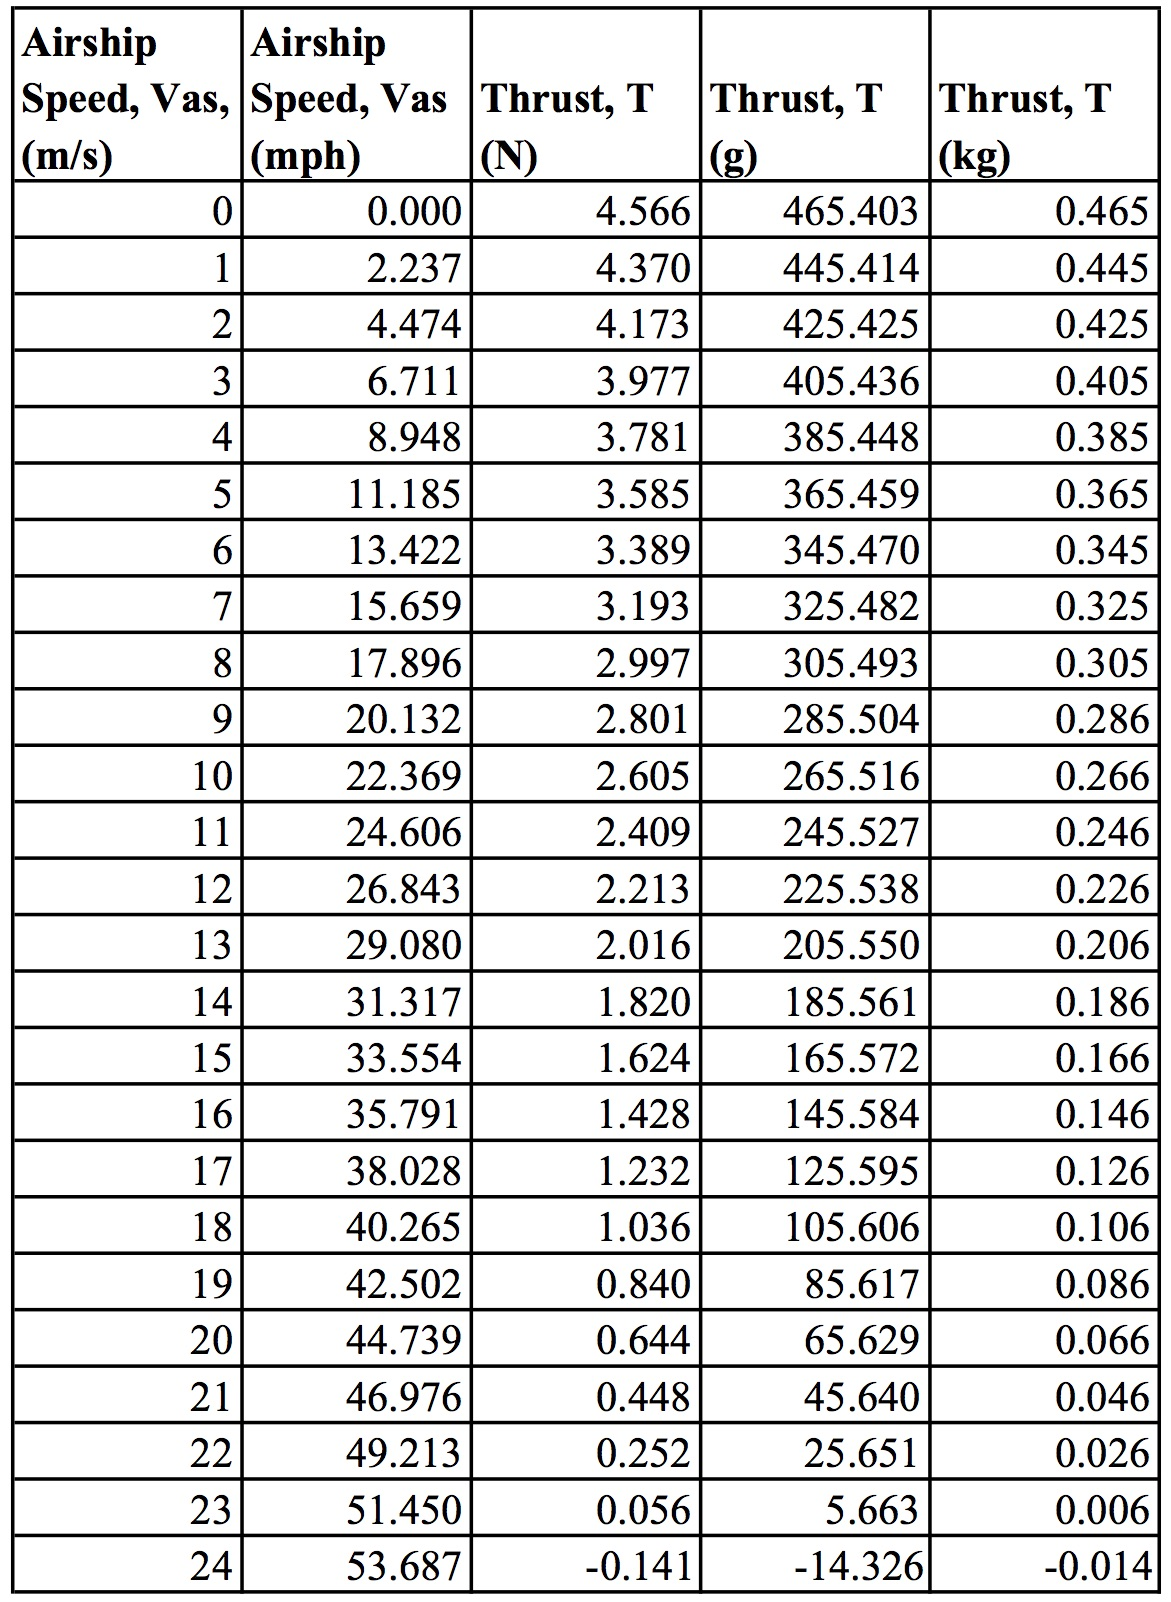
\includegraphics[width=0.75\textwidth]{img/thrust/thrust_table.jpg}
	\label{table:thrustvalues}
\end{table}
\begin{figure}[H]
	\centering
	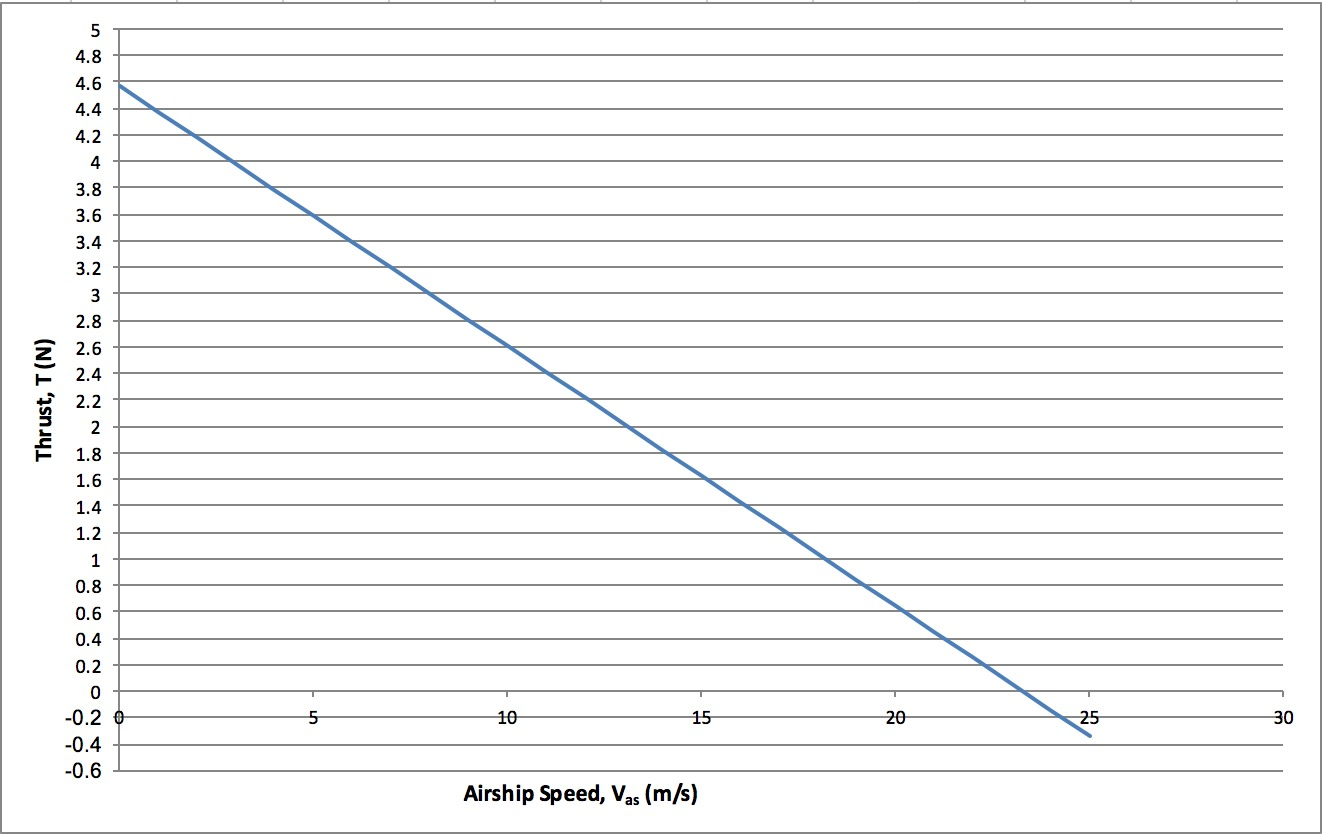
\includegraphics[width=1\textwidth]{img/thrust/thrustours.jpg}
	\caption{Graph of Thrust Plotted Against Airship Speed at 11000rpm With 7", 5" Pitch Diameter Propeller}
	\label{fig:thrusttablours}
\end{figure}
\begin{figure}[H]
	\centering
	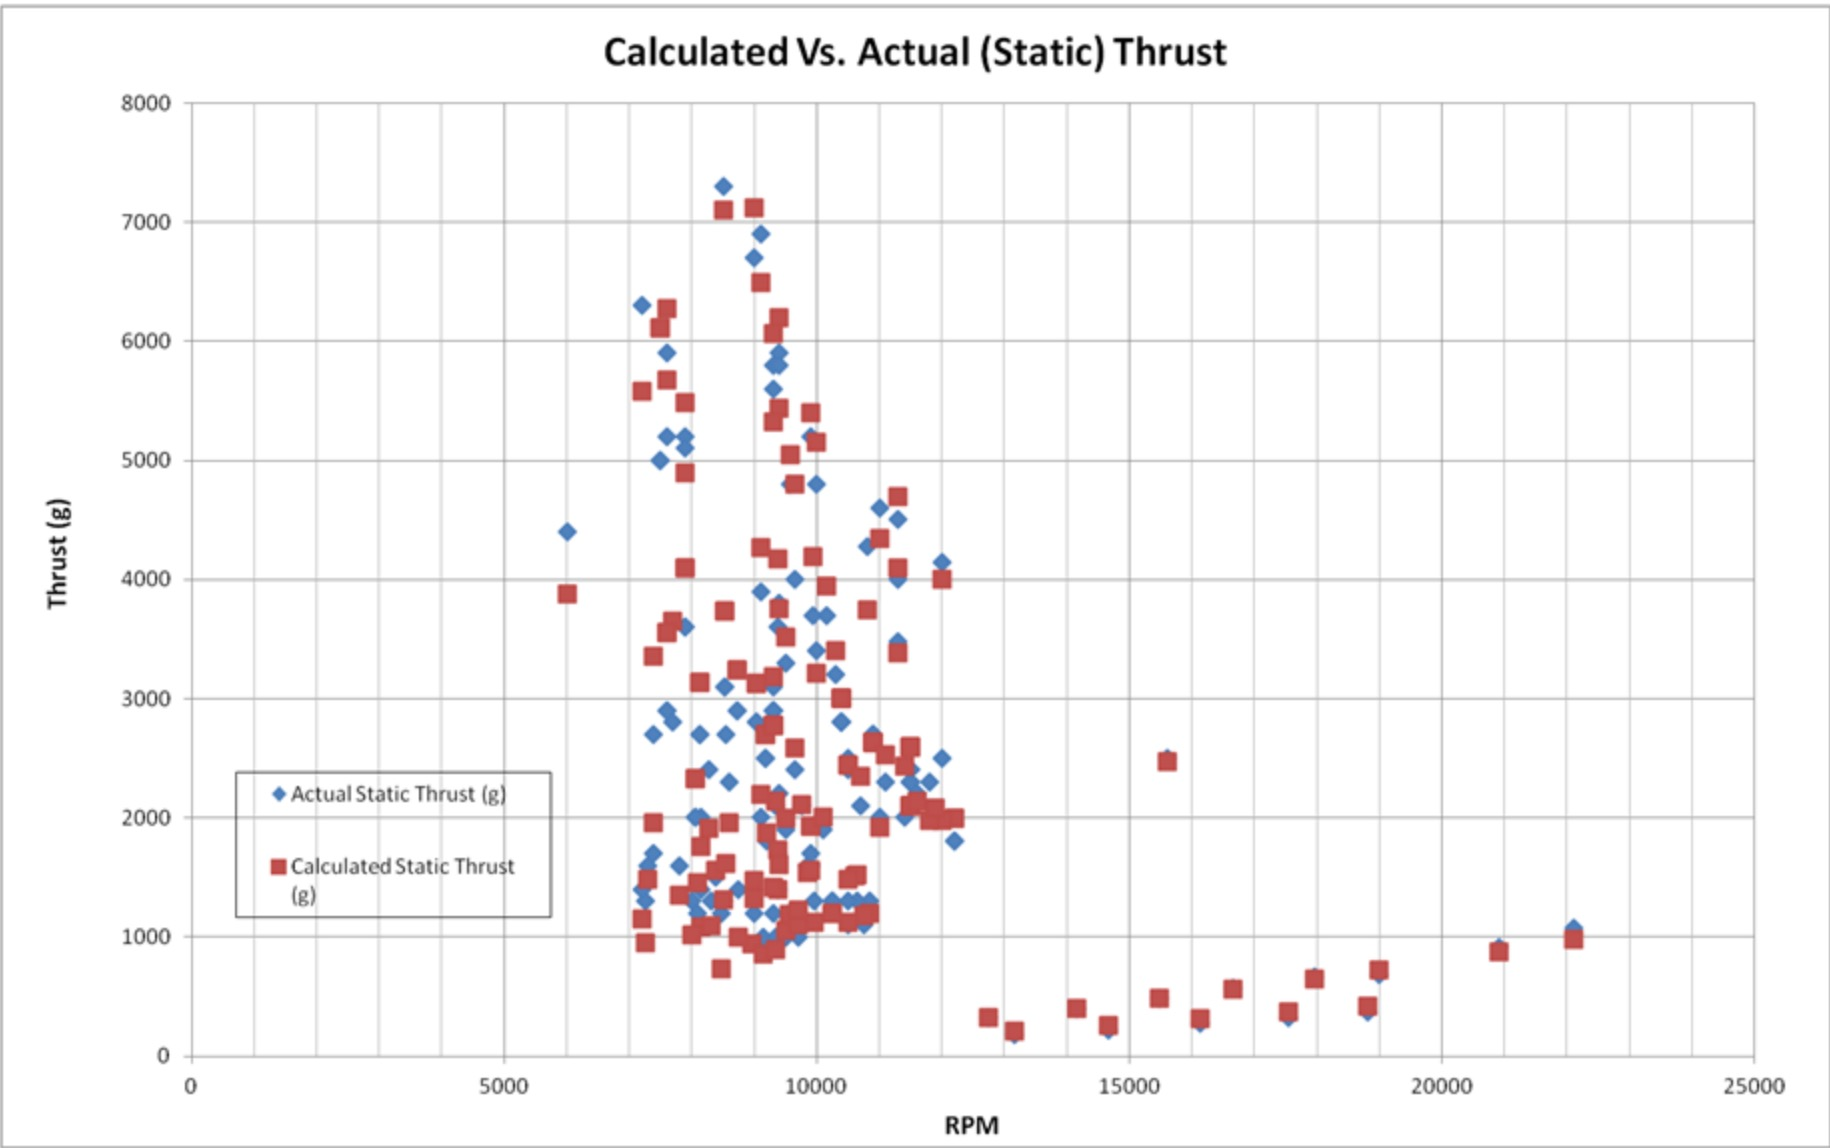
\includegraphics[width=1\textwidth]{img/thrust/thruststatictest.jpg}
	\caption{Test Data from Gabriel Staples Against Experimental Static Thrust Values \cite{thrusteq}}
	\label{fig:thruststatictest}
\end{figure}

\begin{figure}[H]
	\centering
	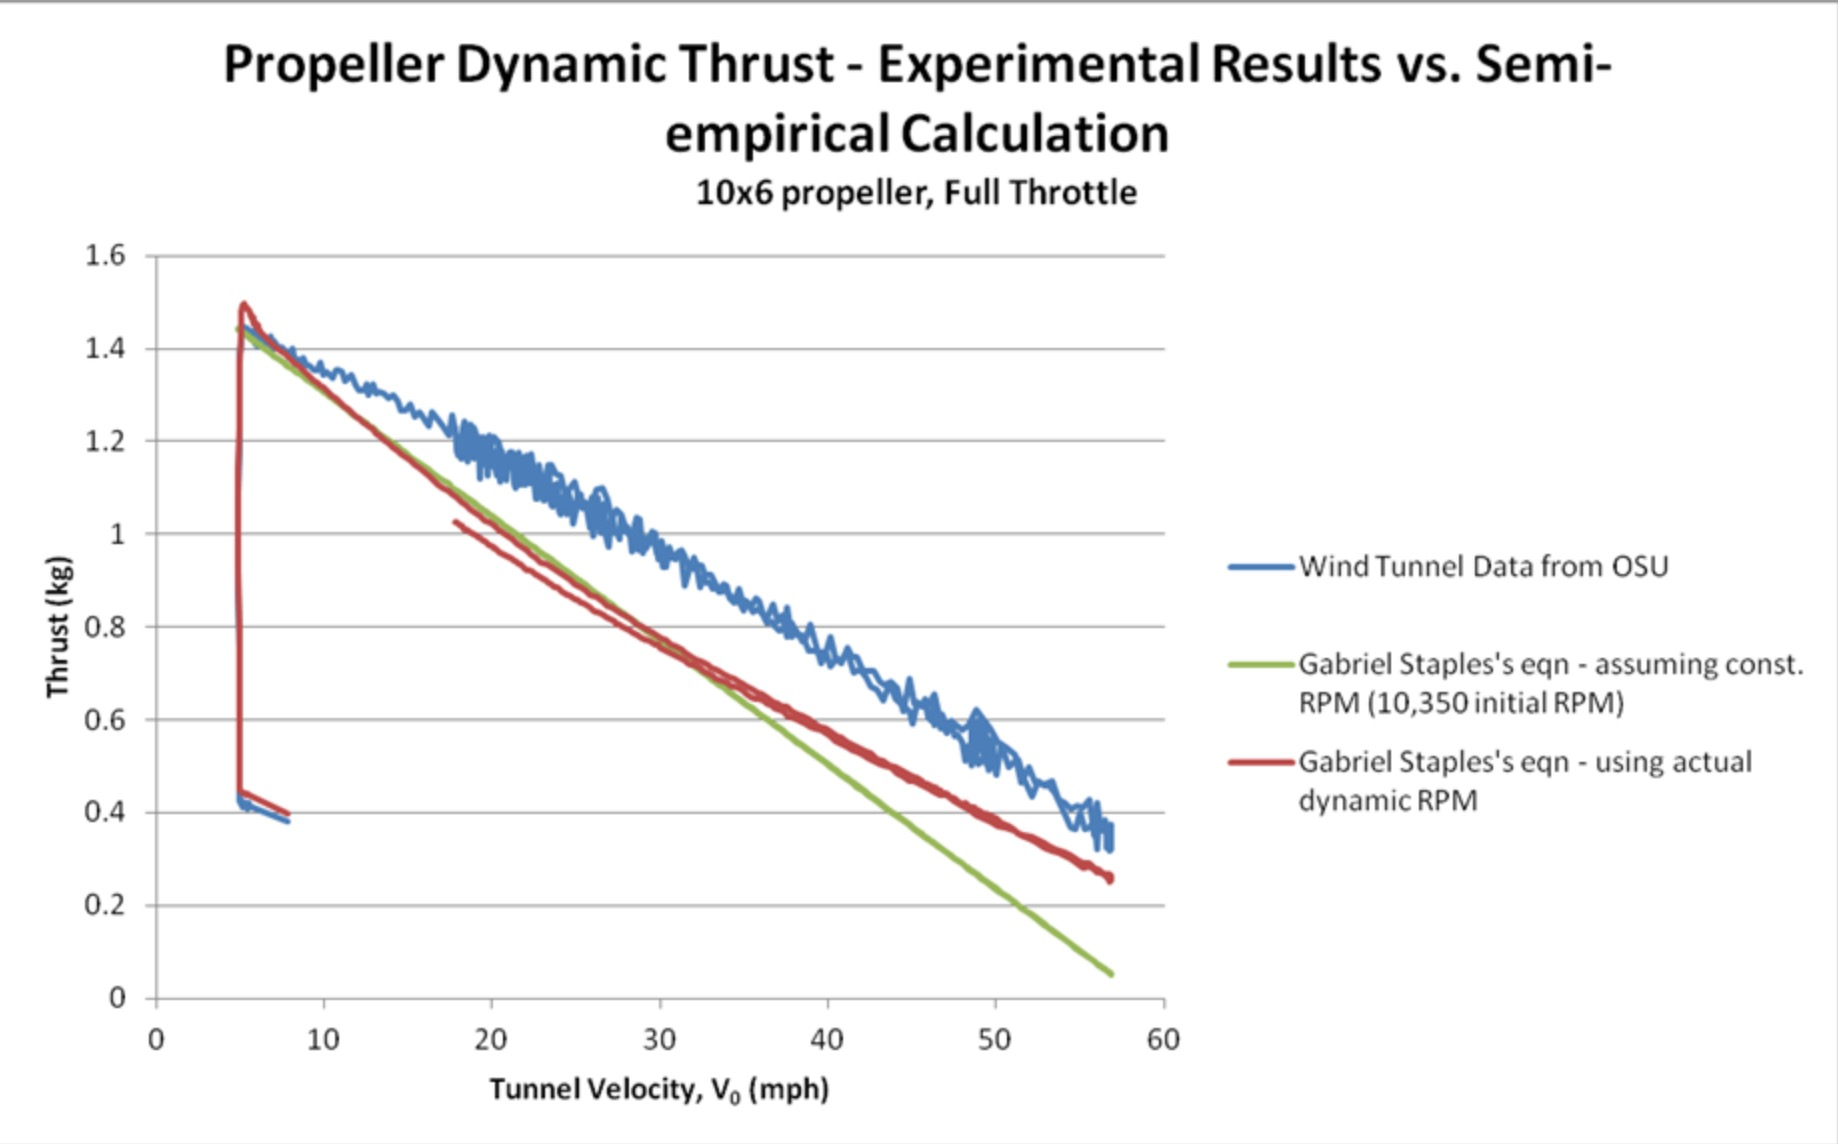
\includegraphics[width=1\textwidth]{img/thrust/thrustdynamictest.jpg}
	\caption{Test Data from Gabriel Staples Against Experimental Dynamic Thrust Values \cite{thrusteq}}
	\label{fig:thrustdynamictest}
\end{figure}

\begin{figure}[H]
	\centering
	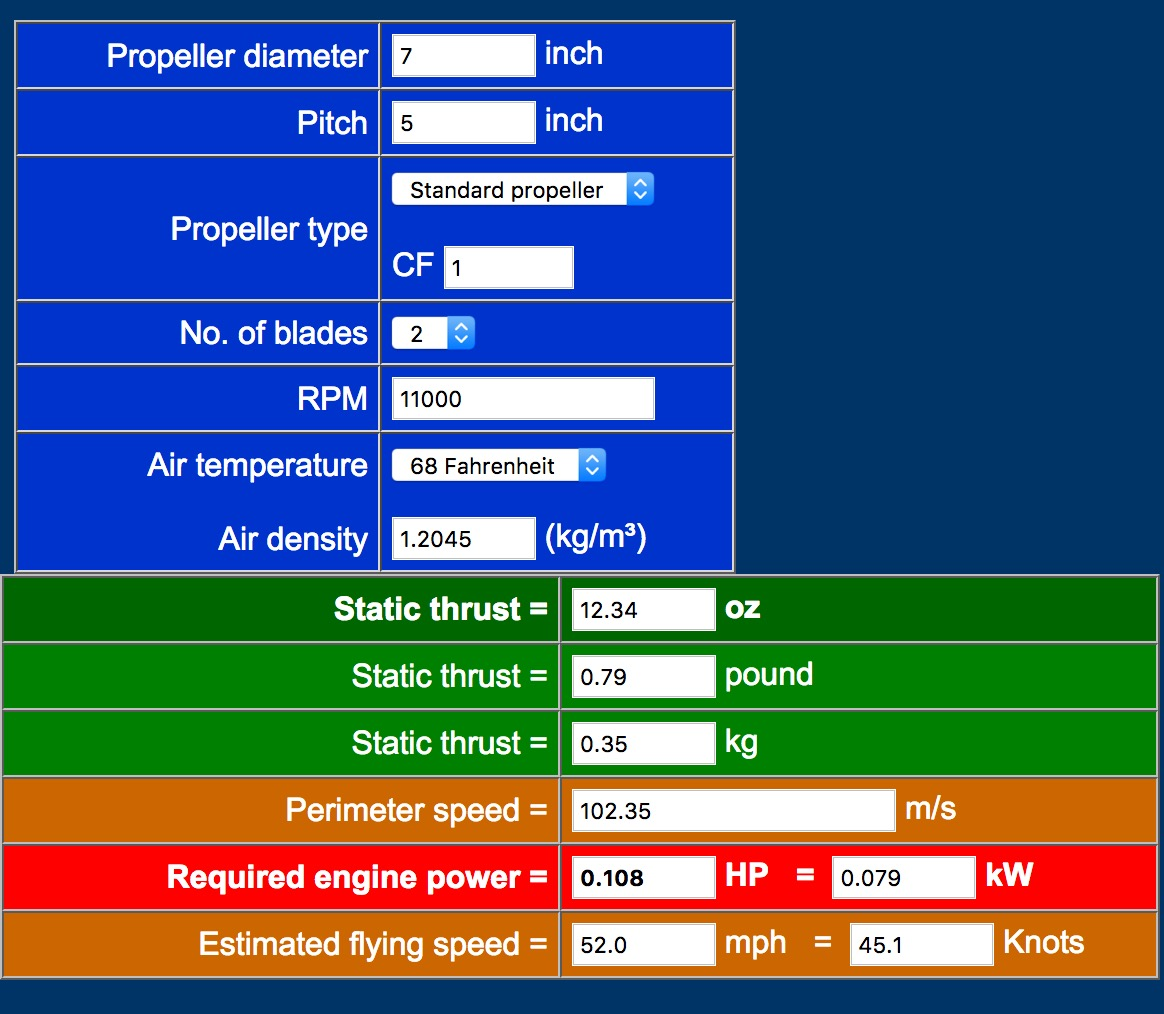
\includegraphics[width=1\textwidth]{img/thrust/thrustcalc.jpg}
	\caption{Sample Thrust Calculation Using On-line Calculator \cite{thrustcalc}}
	\label{fig:thrustcalc}
\end{figure}

\pagebreak

\end{document}